\XtoCBlock{Selector}
\label{block:Selector}
\begin{figure}[H]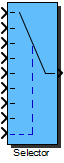
\includegraphics{Selector}\end{figure} 

\begin{XtoCtabular}{Inports}
In0 & Input \#0\tabularnewline
\hline
In1 & Input \#1\tabularnewline
\hline
In2 & Input \#2\tabularnewline
\hline
In3 & Input \#3\tabularnewline
\hline
In4 & Input \#4\tabularnewline
\hline
In5 & Input \#5\tabularnewline
\hline
In6 & Input \#6\tabularnewline
\hline
In7 & Input \#7\tabularnewline
\hline
Select & Input select\tabularnewline
\hline
\end{XtoCtabular}


\begin{XtoCtabular}{Outports}
Out & Selected input signal\tabularnewline
\hline
\end{XtoCtabular}

\subsubsection*{Description:}
Passing through of input signal selected by the select inport:

  Select = 0 (DSP): Out = In0

  Select = 1 (DSP): Out = In1

  ...

  Select = 7 (DSP): Out = In7

% include optional documentation file
\InputIfFileExists{\XcHomePath/Library/General/Doc/Selector_Info.tex}{\vspace{1ex}}{}

\subsubsection*{Implementations:}
\begin{tabular}{l l}
\textbf{FiP8} & 8 Bit Fixed Point Implementation\tabularnewline
\textbf{FiP16} & 16 Bit Fixed Point Implementation\tabularnewline
\textbf{FiP32} & 32 Bit Fixed Point Implementation\tabularnewline
\textbf{Float32} & 32 Bit Floating Point Implementation\tabularnewline
\textbf{Float64} & 64 Bit Floating Point Implementation\tabularnewline
\end{tabular}

\XtoCImplementation{FiP8}
\nopagebreak[0]

8 Bit Fixed Point Implementation

\begin{XtoCtabular}{Inports Data Type}
In0 & int8\tabularnewline
\hline
In1 & int8\tabularnewline
\hline
In2 & int8\tabularnewline
\hline
In3 & int8\tabularnewline
\hline
In4 & int8\tabularnewline
\hline
In5 & int8\tabularnewline
\hline
In6 & int8\tabularnewline
\hline
In7 & int8\tabularnewline
\hline
Select & int8\tabularnewline
\hline
\end{XtoCtabular}

\begin{XtoCtabular}{Outports Data Type}
Out & int8\tabularnewline
\hline
\end{XtoCtabular}

\ifdefined \AddTestReports
\InputIfFileExists{\XcHomePath/Library/General/Doc/Test-Results/Test_Selector_FiP8.tex}{}{}
\fi
\XtoCImplementation{FiP16}
\nopagebreak[0]

16 Bit Fixed Point Implementation

\begin{XtoCtabular}{Inports Data Type}
In0 & int16\tabularnewline
\hline
In1 & int16\tabularnewline
\hline
In2 & int16\tabularnewline
\hline
In3 & int16\tabularnewline
\hline
In4 & int16\tabularnewline
\hline
In5 & int16\tabularnewline
\hline
In6 & int16\tabularnewline
\hline
In7 & int16\tabularnewline
\hline
Select & int8\tabularnewline
\hline
\end{XtoCtabular}

\begin{XtoCtabular}{Outports Data Type}
Out & int16\tabularnewline
\hline
\end{XtoCtabular}

\ifdefined \AddTestReports
\InputIfFileExists{\XcHomePath/Library/General/Doc/Test-Results/Test_Selector_FiP16.tex}{}{}
\fi
\XtoCImplementation{FiP32}
\nopagebreak[0]

32 Bit Fixed Point Implementation

\begin{XtoCtabular}{Inports Data Type}
In0 & int32\tabularnewline
\hline
In1 & int32\tabularnewline
\hline
In2 & int32\tabularnewline
\hline
In3 & int32\tabularnewline
\hline
In4 & int32\tabularnewline
\hline
In5 & int32\tabularnewline
\hline
In6 & int32\tabularnewline
\hline
In7 & int32\tabularnewline
\hline
Select & int8\tabularnewline
\hline
\end{XtoCtabular}

\begin{XtoCtabular}{Outports Data Type}
Out & int32\tabularnewline
\hline
\end{XtoCtabular}

\ifdefined \AddTestReports
\InputIfFileExists{\XcHomePath/Library/General/Doc/Test-Results/Test_Selector_FiP32.tex}{}{}
\fi
\XtoCImplementation{Float32}
\nopagebreak[0]

32 Bit Floating Point Implementation

\begin{XtoCtabular}{Inports Data Type}
In0 & float32\tabularnewline
\hline
In1 & float32\tabularnewline
\hline
In2 & float32\tabularnewline
\hline
In3 & float32\tabularnewline
\hline
In4 & float32\tabularnewline
\hline
In5 & float32\tabularnewline
\hline
In6 & float32\tabularnewline
\hline
In7 & float32\tabularnewline
\hline
Select & int8\tabularnewline
\hline
\end{XtoCtabular}

\begin{XtoCtabular}{Outports Data Type}
Out & float32\tabularnewline
\hline
\end{XtoCtabular}

\ifdefined \AddTestReports
\InputIfFileExists{\XcHomePath/Library/General/Doc/Test-Results/Test_Selector_Float32.tex}{}{}
\fi
\XtoCImplementation{Float64}
\nopagebreak[0]

64 Bit Floating Point Implementation

\begin{XtoCtabular}{Inports Data Type}
In0 & float64\tabularnewline
\hline
In1 & float64\tabularnewline
\hline
In2 & float64\tabularnewline
\hline
In3 & float64\tabularnewline
\hline
In4 & float64\tabularnewline
\hline
In5 & float64\tabularnewline
\hline
In6 & float64\tabularnewline
\hline
In7 & float64\tabularnewline
\hline
Select & int8\tabularnewline
\hline
\end{XtoCtabular}

\begin{XtoCtabular}{Outports Data Type}
Out & float64\tabularnewline
\hline
\end{XtoCtabular}

\ifdefined \AddTestReports
\InputIfFileExists{\XcHomePath/Library/General/Doc/Test-Results/Test_Selector_Float64.tex}{}{}
\fi
